\section{How to Create Plots?}

We will now show several possibilities for plotting, using different
technologies. For each of the following technologies, we give an example to
provide an idea to the reader of how the work with this technology might look
like. The examples are in alphabetical order of the technology name; afterwards
we will only look closer into \texttt{pgfplots}.

\subsection{Gnuplot}

\toolname{Gnuplot} is a portable command-line driven graphing utility for
various platforms.  It is freely available under a free license.  Originally
created in 1986, it is a tool that allows the user to visualize mathematical
functions and data interactively~\cite{WilliamsKelley2016}.  The documentation
and many examples can be found on the project's
homepage\footnote{\href{http://www.gnuplot.info}{http://www.gnuplot.info}}.

\toolname{Gnuplot} can produce its output in many different formats: directy on
screen, or as graphics file, include PNG, EPS, SVG, JPEG, and many more; it is
also capable of producing \LaTeX{} code that can be included directly in
\LaTeX{} documents.

\subsection{pgfplots}

\toolname{Pgfplots} is a package for \TeX{} and \LaTeX{} using Till Tantau's
package \toolname{pgf/Ti\textit{k}Z}~\cite{Feuersaenger2016}.  It supports line
plots, scatter plots, bar plots, histogram plots, box plots, and many more and
is able to do 2D and 3D plots without needing an external tool installed
(contrary to \toolname{PSTricks}).

The input file is of the structure as a standard \TeX{} or \LaTeX{} file.
Consider the example code in Listing~\ref{lst:pgfplots-example}, which is taken
from the \toolname{pgfplots} manual~\cite{Feuersaenger2016}.  It uses a data set
that comes with \toolname{pgfplots} to plot the curve that can be seen in
Figure~\ref{fig:pgfplots-example}.

\begin{listing}[H]
  \inputminted{latex}{../examples/pgfplots-example.tex}
  \caption{Example code for \toolname{pgfplots} (taken
    from~\cite{Feuersaenger2016})}
  \label{lst:pgfplots-example}
\end{listing}
\begin{figure}[!t]
  \centering
  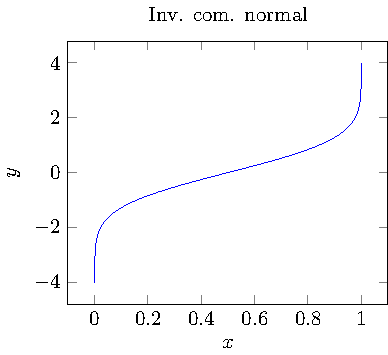
\includegraphics{pgfplots-example}
  \caption{Resulting diagram from the code in Lst.~\ref{lst:pgfplots-example}}
  \label{fig:pgfplots-example}
\end{figure}

\subsection{PSTricks}

\toolname{PSTricks} is the name of an extensive collection of packages to create
PostScript that is usable from \TeX~\cite{Zandt2007}.  In order to use
PostScript, one needs to use the tool chain \texttt{latex} $\rightarrow$
\texttt{dvips} $\rightarrow$ \texttt{ps2pdf} in order to create PDFs; this
limitation can be overcome by using either the \toolname{pst-pdf} or the
\toolname{pdftricks} package, that create PDF directly.

As \toolname{PSTricks} uses PostScript, it has access to the full power of this
(Turing complete) language.  For creating plots, the \toolname{pst-plot}
package~\cite{Voss2016a} exists.  In Listing~\ref{lst:pstricks-example} is an
example of a simple plot with this package; the result can be seen in
Figure~\ref{fig:pstricks-example}.  The code was taken from the
\toolname{PSTricks} gallery\footnote{\href{http://pstricks.tug.org}%
{http://pstricks.tug.org}}.

\begin{listing}[H]
  \inputminted{latex}{../examples/pstricks-example.tex}
  \caption{Example code for \toolname{PSTricks}}
  \label{lst:pstricks-example}
\end{listing}
\begin{figure}[!t]
  \centering
  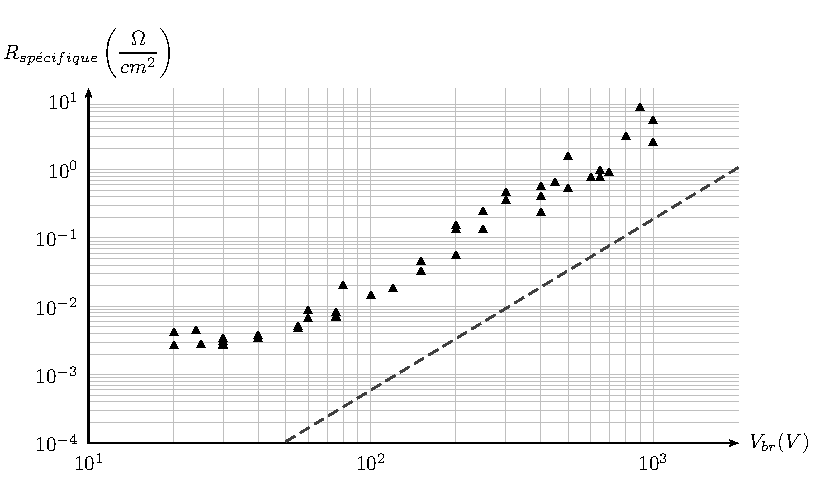
\includegraphics[width=\linewidth]{pstricks-example}
  \caption{Resulting diagram from the code in Lst.~\ref{lst:pstricks-example}}
  \label{fig:pstricks-example}
\end{figure}

A rich introduction in the functionality of \toolname{PSTricks} that goes far
beyond plotting can be found in the German book \enquote{PSTricks -- Grafiken
mit PostScript für \TeX{} und \LaTeX{}} by Herbert Voß~\cite{Voss2016}.

\subsection{R and Sweave}

\toolname{R} is a well-known language for statistical computing and
graphics~\cite{Ihaka1998}.  A huge variety of modules is available at the
Comprehensive R Archive Network (CRAN)\footnote{%
  \href{https://cran.r-project.org}{https://cran.r-project.org}}.  One of these
modules is called \toolname{Sweave}, initially developed by Friedrich
Leisch~\cite{Leisch2002}.  It combines \LaTeX{} and \toolname{R} in the style of
literate programming—a concept developed by Donald E\@. Knuth~\cite{Knuth1992}.
A simple introduction was given by Uwe Ziegenhagen in his German article
\enquote{Datenanalyse mit Sweave, \LaTeX{} und R}~\cite{Ziegenhagen2010}.

\begin{listing}[H]
  \inputminted{latex}{../examples/sweave-example.Snw}
  \caption{Plot the exchange rate between \euro{} and \$ dynamically using
    \toolname{Sweave}}
  \label{lst:sweave-example}
\end{listing}

\begin{figure}[!t]
  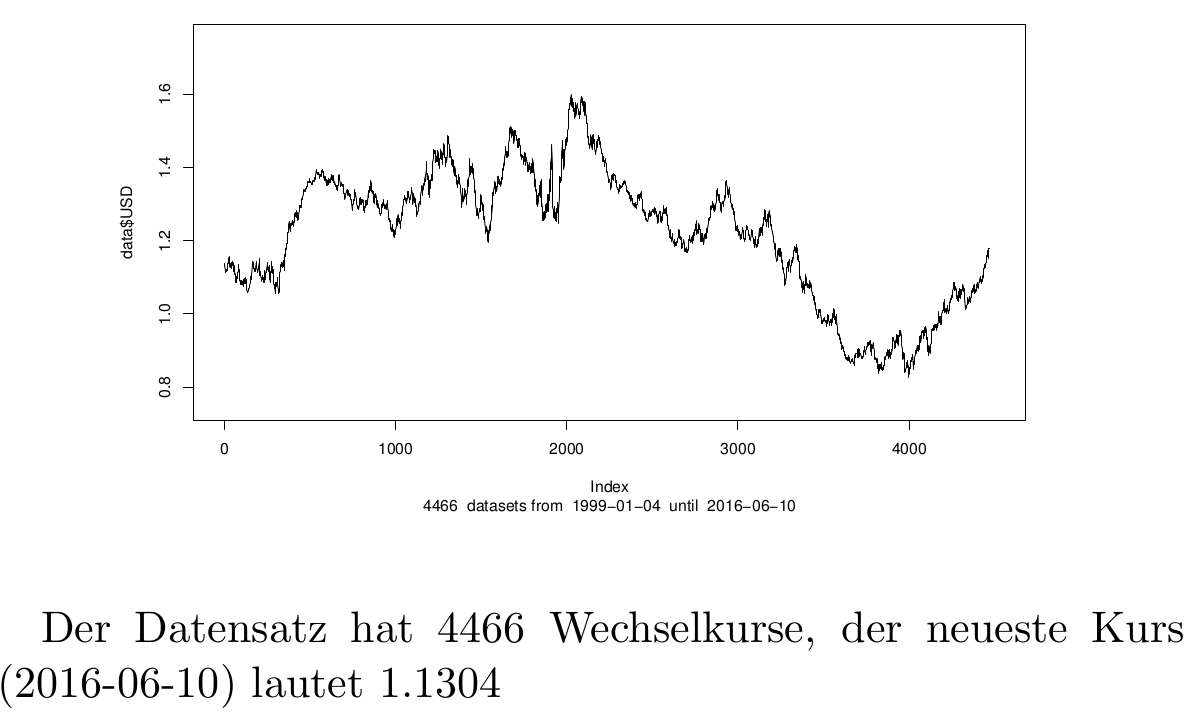
\includegraphics[width=\linewidth]{sweave-example}
  \caption{Screenshot of the \toolname{Sweave} example in
    Lst.~\ref{lst:sweave-example}}
  \label{fig:sweave-example}
\end{figure}

In order to use \toolname{Sweave}, one needs to write a document like shown in
Listing~\ref{lst:sweave-example}.  By convention, the filename suffix is not
\texttt{*.tex} but \texttt{*.Snw}; this is important, because the \texttt{*.tex}
file will be create automatically.  A syntax highlighting mode is available for
the editor VIM\@.  After writing the file, one needs to start \toolname{R},
e.g., a \toolname{R} interactive shell.  With the command
\mintinline{R}{Sweave("filename.Snw")} the \toolname{R} code will be processed
and a \texttt{*.tex} file will be created, which can then be processed by, e.g.,
\hologo{pdfLaTeX}.

The example in Listing~\ref{lst:sweave-example} loads the exchange rates between
\euro{} and \$ from the homepage of the European Central Bank and plots it. The
output can be seen in Figure~\ref{fig:sweave-example}.
